
\section{Wprowadzenie}
Przykłady obliczeń Python i Matlab zostały zaczerpnięte z \cite{ossowski2023}.
\textbf{Pełen kod dostępny na github:} https://github.com/piotrHeinzelman/inz/tree/main/MixedProj/01.polyfit
w przypadku Matlab i Python korzystam z dostępnych funkcji, w przypadku Java obliczam wg. wzoru ~\ref{eq:linearregresion}. Obliczenia różnymi metodami dają zbliżone wyniki, więc zakładam że moje implementacje są poprawne. 

 
W pracy tam gdzie możliwe staram się wykorzystać dostarczone funkcje liczące. I tak dla Matlab i dla Python wykorzystałem zaimplementowaną funkcję "polyfit". W kodzie Java musiałem sam zaimplementować funkcję liczącą dla porównania wydajności. W programach nie porównuję czasu ładowania i przygotowania danych ponieważ chcę wykonywać obliczenia dla tych samych wartości czytanych z tych samych plików, natomiast nie jest moim celem optymalizacja wczytywania danych z pliku.

\newpage
\section{Prowadzenie badania}
Programy w kolejnych językach uruchamiam poniższym kodem:

\begin{lstlisting}[ basicstyle=\tiny]
./matRun >> output.txt
./pyRun  >> output.txt
./javaRun >> output.txt

//matRun
echo "--- Matlab app start: ---"
/usr/local/MATLAB/R2024a/bin/matlab  -nodisplay -nosplash -nodesktop -batch 'run matlab.m'

//pyRun
echo "--- Python app start: --- "
python main.py

// javaRun
javac Main.java 
echo "--- Java app start: ---"
java Main
\end{lstlisting}


\section{Kod realizujący obliczenia}


\begin{lstlisting}[ basicstyle=\tiny]
//                  --- MATLAB ---

    a = polyfit(x,y,1);

//                  --- Python --- 

    a = np.polyfit(x,y,1)

//                  ---  Java --- 

     for (int i = 0; i < x.length; i++) {
            xsr += x[i];
            ysr += y[i];
        }
        xsr = xsr / x.length;
        ysr = ysr / y.length;

        for (int i = 0; i < x.length; i++) {
            sumTop += ((x[i] - xsr) * (y[i] - ysr));
            sumBottom += ((x[i] - xsr) * (x[i] - xsr));
        }
        w1 = sumTop / sumBottom;
        w0 = ysr - w1 * xsr;

//               --- C++ ---

      for ( int i=0; i<len; i++ ){
         xsr +=  X[i];
         ysr +=  Y[i];
      }
   xsr=xsr / len; ysr=ysr / len;
   double sumTop=0.0;
   double sumBottom=0.0;

      for ( int i=0;i<len;i++ ){ //  xtmp = X[i]-sr ! ;
       sumTop   += ((X[i]-xsr)*(Y[i]-ysr));
      sumBottom += ((X[i]-xsr)*(X[i]-xsr));
      }
      w1 = sumTop / sumBottom;
      w0 = ysr -(w1 * xsr) ;
        
.   
\end{lstlisting}

\newpage
\section{Uzyskane wyniki}

\begin{figure}[h]
    	\centering 
            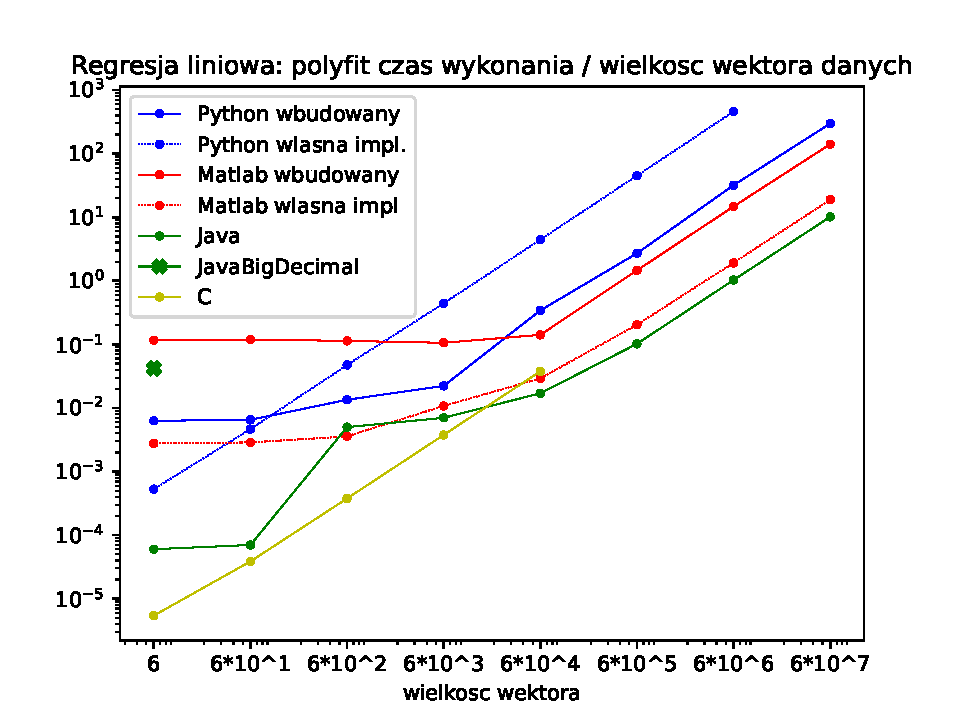
\includegraphics[width=0.70\linewidth]{gfx/fig01.pdf} 
\end{figure} 
\begin{figure}[h]
    \begin{subfigure}{.5\textwidth}
    	\centering 
            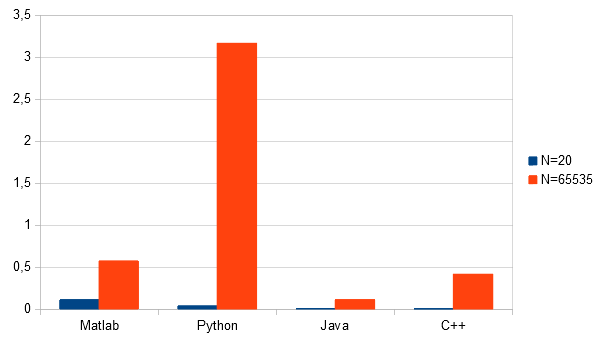
\includegraphics[width=0.95\linewidth]{gfx/01a.png} 
    \end{subfigure} %
    \begin{subfigure} {.5\textwidth}
    	\centering 
            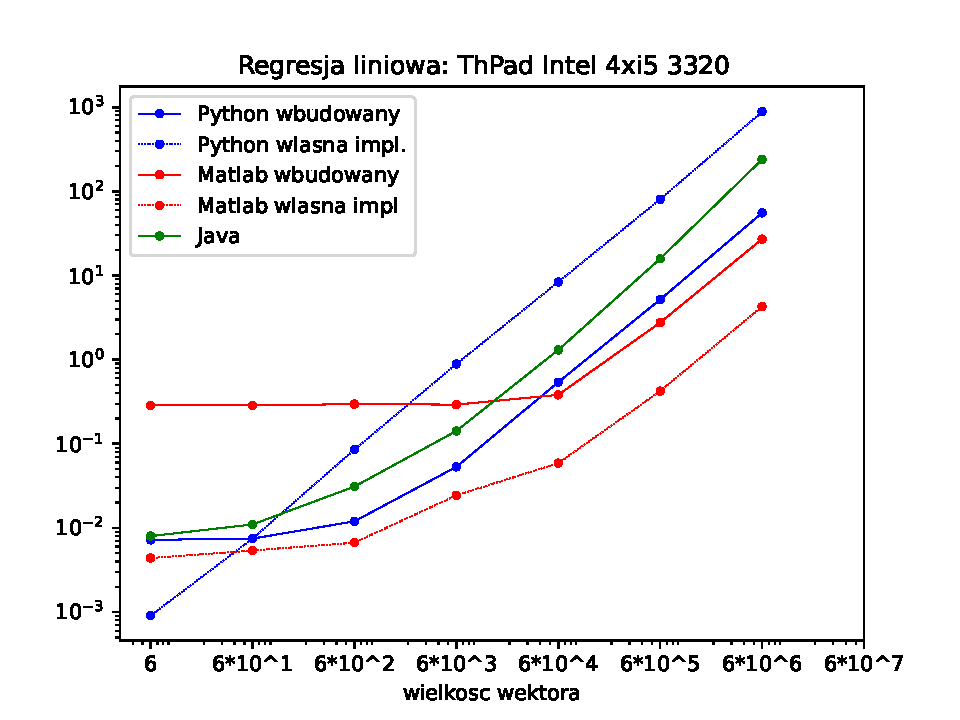
\includegraphics[width=0.95\linewidth]{gfx/fig01_PC2.pdf} 
    \end{subfigure} 
    \caption{Porównanie czasów obliczania regresji liniowej}
\end{figure} 